\section{Computer Networks}

    \begin{figure}[H]
        \centering
        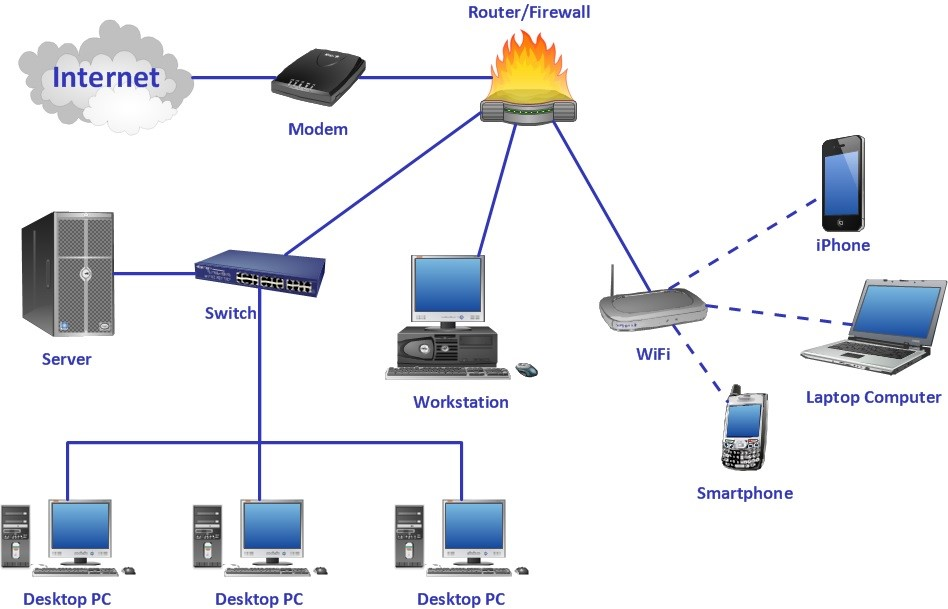
\includegraphics[width=0.7\textwidth]{images/e073f6.jpg}

        \caption{Computer Networking. From: \url{https://www.learnelectronicsindia.com/post/collection-of-computers}.}
        \label{fig:intranet}
    \end{figure}

    Maybe the most famous kind of networks, Computer Networks are composed of computers some other form of hardware communicating between them. The links are either physical cables or some form of wireless communication protocol. These networks are the base of the Internet.

    Different from previous networks, Computer Netorks are physical and can't be fully represented with drawings. However, if you consider some limited aspects of the network, they might still be useful to analyze the topology of a specific netowrk, like \cref{fig:intranet}.
